\documentclass{article}

% PACKAGES
\usepackage{pgfplots}
\pgfplotsset{compat=1.18}
\usepackage[margin=2cm]{geometry}
\usepackage{graphicx}
\usepackage{float}
\usepackage{caption}
\usepackage{subcaption}
\usepackage{amsmath}
\usepackage{booktabs}
\usepackage{eurosym}

\usepackage[colorlinks=true, allcolors=black]{hyperref}
\usepackage{balance}

% INFORMATIONS
\title{Electric vehicle fleet strategies for smart participation in primary frequency reserve}
\author{Amorotti Lucas, Retailleau Mathieu, Aurelian Andrei Panait \\ Wenjun Wang, Feihong Li}
\date{January 2026}

\begin{document}

%%%%%%%%%%%%%%%%%%%%%%%%%%%%%%%%%%%%%%
% PAGE DE GARDE
%%%%%%%%%%%%%%%%%%%%%%%%%%%%%%%%%%%%%%
\begin{titlepage}
    \centering
    
    % LOGO MINES PSL
    \begin{figure}[H]
        \centering
        
\includegraphics[width=0.6\textwidth]{pictures/logo_mines_PSL.png} 
    \end{figure}

    \vspace*{1cm}

    {\Huge \textbf{Electric vehicle fleet strategies for smart participation in primary frequency reserve} \par}
    
    \vspace{1.5cm}
    
    {\Large \textbf{Authors:}} \\
    {\Large Amorotti Lucas \\ Retailleau Mathieu \\ Aurelian Andrei Panait \\ Wenjun Wang\\ Feihong Li\par}
    
    \vspace{1cm}
    {\Large January-February 2026 \par}
    
    \vfill
    
    {\Large \textbf{Supervised by}}\\[0.2cm]
    {\Large Pierre Dumont}\\
    {\Large PhD}
    
    \vfill

\end{titlepage}

%%%%%%%%%%%%%%%%%%%%%%%%%%%%%%%%%%%%%%
% ABSTRACT & TOC
%%%%%%%%%%%%%%%%%%%%%%%%%%%%%%%%%%%%%%
\clearpage

\begin{abstract}
\large % Police agrandie pour l'abstract
This project investigates the participation of electric vehicle fleets in primary frequency containment reserves (FCR). Using publicly available grid frequency data, the regulating power requested by the transmission system operator is analysed. Several dispatch strategies are evaluated. Results show that a "Smart" dispatch strategy increases energy efficiency to 95\% and reduces on-board charger operating time to roughly 7\%. However, this strategy induces higher battery degradation (+7.5\%) compared to a uniform distribution (+2.8\%) due to current concentration. Economic analysis confirms a positive net revenue of approximately €40/EV/month, accounting for battery depreciation.
\end{abstract}

\clearpage
\tableofcontents
\clearpage

%%%%%%%%%%%%%%%%%%%%%%%%%%%%%%%%%%%%%%
% CONTENU PRINCIPAL
%%%%%%%%%%%%%%%%%%%%%%%%%%%%%%%%%%%%%%
\twocolumn

\section{Introduction}
The transition towards a low-carbon energy sector is driving a massive integration of variable renewable energy sources (VRES), such as wind and solar photovoltaics. While essential for decarbonization, these sources introduce significant volatility and reduce the natural inertia of the power system, making the balance between generation and consumption harder to maintain. In this context, maintaining grid frequency stability has become a critical challenge for Transmission System Operators (TSOs). Primary Frequency Containment Reserves (FCR) constitute the first line of defense, providing fast, automatic power adjustments to stabilize the grid frequency in the seconds following a deviation.

Battery Energy Storage Systems (BESS) are particularly well-suited for FCR provision due to their extremely fast response times compared to thermal generators. Among these assets, Electric Vehicles (EVs) represent a vast, distributed, and often underutilized storage capacity. With the advent of Vehicle-to-Grid (V2G) technology, EVs can not only draw power but also inject it back into the grid. When aggregated, a fleet of EVs can act as a "virtual power plant," offering a flexible solution to grid stability issues without requiring additional centralized infrastructure.

However, the participation of EVs in FCR raises complex technical and economic trade-offs. The constant micro-cycling required by frequency regulation impacts the battery State-of-Charge (SOC) and may accelerate ageing, potentially compromising the primary function of the vehicle: mobility. This project investigates these challenges by modelling a fleet of EVs under real frequency data constraints from 2019 and 2021. We evaluate different dispatch strategies to optimize the balance between power conversion efficiency, availability constraints, and battery degradation.

\section{Frequency Containment Reserve Modelling}

\subsection{TSO regulation law}
The participation in FCR is governed by a proportional control law defined by the TSO. The power response $P_{RE}(t)$ required from a Reserve Entity (RE) is a function of the instantaneous grid frequency $f(t)$ and the contracted power capacity $P_{bid}$:

\begin{equation}
    P_{RE}(t) = k \cdot P_{bid} \cdot (f(t) - f_n) + P_c
\end{equation}

Where:
\begin{itemize}
    \item $f_n = 50$ Hz is the nominal grid frequency.
    \item $k$ is the droop coefficient, typically set to $5 \text{ Hz}^{-1}$ in the Continental Europe synchronous area.
    \item $P_{bid}$ is the reserved power capacity (kW).
    \item $P_c$ is a command setpoint (assumed to be 0 for pure FCR).
\end{itemize}

\subsection{Distribution and Analysis of Regulating Power (Q1-Q2)}

\subsubsection{Computed Distribution}
To assess the actual solicitation of the fleet, we analyzed grid frequency data over a one-month period. By assuming $P_c=0$, we computed the normalized regulating power distribution defined as $P_{RE}^{p.u.}(t) = \frac{P_{RE}(t)}{P_{bid}}$. Figure \ref{fig:q1_dist} displays the resulting histogram.

\begin{figure}[H]
    \centering
    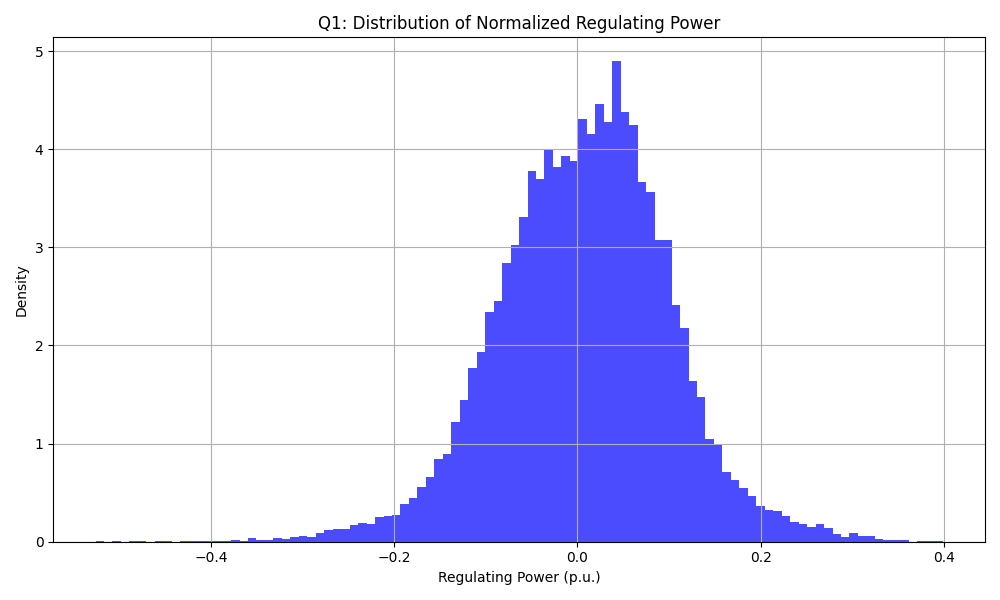
\includegraphics[width=\linewidth]{pictures/q1_distribution.png}
    \caption{Distribution of Normalized Regulating Power (Q1).}
    \label{fig:q1_dist}
\end{figure}

\subsubsection{Observations}
The distribution follows a Gaussian-like shape strictly centered at 0 p.u. This indicates a balanced regulation effort over the month, with the fleet spending roughly equal time in charging mode ($P_{RE} > 0$, corresponding to $f(t) > 50$ Hz) and discharging mode ($P_{RE} < 0$, corresponding to $f(t) < 50$ Hz).

\subsubsection{Interpretation and Magnitude (Q2)}
Regarding the magnitude of the regulating power, the histogram reveals that the signal rarely reaches the saturation limits of $\pm 1$ p.u. The vast majority of data points lie within the $\pm 0.4$ p.u. range.

This behaviour is explained by the stability of the European grid. Deviations resulting from the instantaneous imbalance between production and consumption are continuous but typically remain small (within $\pm 0.2$ Hz). The EV fleet acts as a stabilizing counter-force to these deviations: reacting within seconds to "contain" the frequency. The fact that the normalized power remains low implies that the full power capacity ($P_{bid}$) is effectively reserved for rare, critical grid incidents rather than routine balancing.

\section{Impact on Single Electric Vehicle}

\subsection{SOC Deviation Analysis (Q3)}

\subsubsection{Methodology}
The state-of-charge (SOC) evolution is governed by the time integral of the regulating power. In the absence of active energy management (i.e., assuming $P_c=0$), the SOC is driven solely by the stochastic fluctuations of the grid frequency. To quantify this drift, we simulated the SOC deviation of a single vehicle ($E_{batt}=46$ kWh) over rolling time windows of 4, 8, 12, and 24 hours.

\subsubsection{Computed Deviation}
Figure \ref{fig:q3_dev} presents the statistical distribution of SOC deviations for these varying durations.

\begin{figure}[H]
    \centering
    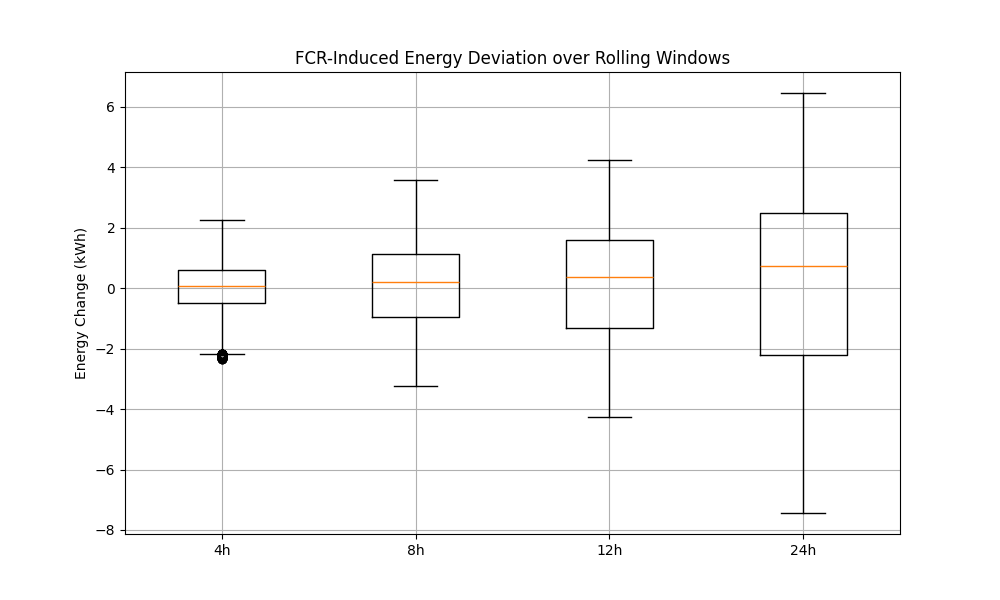
\includegraphics[width=\linewidth]{pictures/q3_rolling_soc_deviation.png}
    \caption{SOC Deviation Distribution over Rolling Windows (Q3).}
    \label{fig:q3_dev}
\end{figure}

\subsubsection{Observations}
The results highlight the "random walk" behaviour inherent to integrating a stochastic signal.
For short durations (4 hours), the deviation is minimal: the interquartile range is confined within $\pm 1\%$, and extrema rarely exceed $\pm 3\%$. However, the dispersion increases mechanically with time. For a 24-hour window, the deviation spreads significantly, with potential drifts exceeding $\pm 10\%$ in extreme cases.

\subsection{Feasibility of Continuous Participation (Q4)}
Based on these observations, we can assess the operational feasibility:

For short contracting blocks (4 to 8 hours), participation is strictly reasonable. The induced energy drift is negligible compared to the total battery capacity, leaving sufficient margins for the user's mobility needs.

Conversely, continuous participation over 24 hours without supervision is risky. The accumulated drift could lead to battery saturation (reaching 100\% or 0\% SOC), forcing the vehicle to stop providing reserves or compromising the user's ability to drive. Therefore, long-term participation requires either an active rebalancing strategy ($P_c \neq 0$) or the limitation of contracts to short 4-hour blocks.

\section{Fleet Dispatch Strategies}

\subsection{Efficiency Analysis (Q5-Q6)}

\subsubsection{Methodology}
We evaluated two dispatch strategies to distribute the regulating power $P_{RE}(t)$ among $N$ vehicles:
\begin{itemize}
    \item \textbf{Uniform Strategy:} Power is shared equally ($P_{i} = P_{RE}/N$). Mathematically, as the total bid scales with $N$, the power per vehicle remains constant regardless of fleet size.
    \item \textbf{Smart Strategy:} The aggregator concentrates power on a subset of vehicles to operate them near optimal efficiency, leaving others idle.
\end{itemize}

\subsubsection{Results and Interpretation}
Figure \ref{fig:q6_eff} compares the efficiency of both strategies.

\begin{figure}[H]
    \centering
    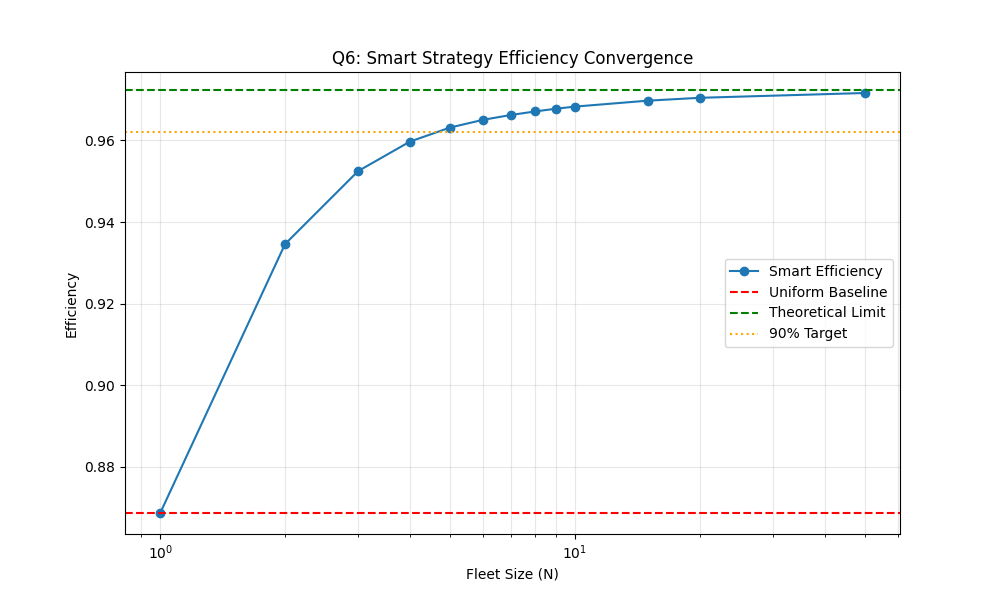
\includegraphics[width=\linewidth]{pictures/q6_efficiency_convergence.png}
    \caption{Efficiency convergence. The Uniform strategy (red dashed) is constant ($\approx 85.9\%$) as expected. The Smart strategy (blue) converges to $\approx 95\%$.}
    \label{fig:q6_eff}
\end{figure}

The \textbf{Uniform strategy efficiency is independent of fleet size}, acting as a baseline. The \textbf{Smart strategy} leverages the statistical diversity of a larger fleet to minimize conversion losses. The convergence threshold to achieve 90\% of the gain is reached at approximately $N_0 \approx 20$ vehicles.

\subsection{On-Board Charger Operating Time (Q7)}
The Smart strategy also minimizes the active time of power electronics. We define the operating time ratio $t_{op}$ as the duration a vehicle provides non-zero power normalized by the total simulation time.

\begin{figure}[H]
    \centering
    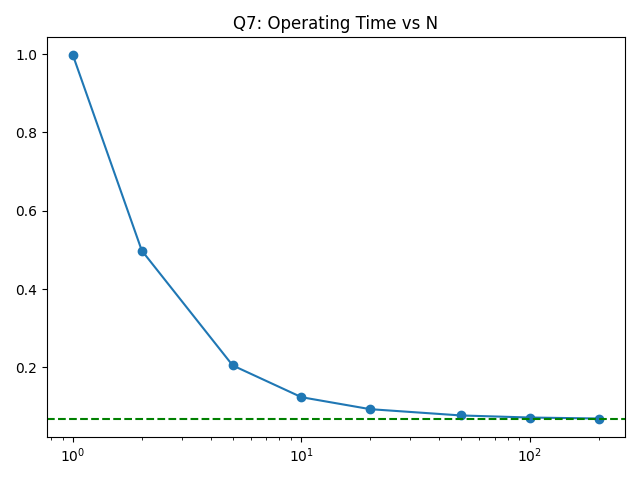
\includegraphics[width=\linewidth]{pictures/q7_operating_time.png}
    \caption{Reduction of Average OBC Operating Time (Q7).}
    \label{fig:q7_time}
\end{figure}

As shown in Figure \ref{fig:q7_time}, while the uniform strategy requires OBCs to be active 100\% of the time (tracking small deviations), the Smart strategy allows OBCs to rest when not needed. For a large fleet ($N \to \infty$), the average operating time converges to a theoretical limit $t_{op}^{\infty} \approx 6.7\%$. This drastic reduction implies significantly lower thermal stress and potentially longer lifespan for the power electronics.


\subsection{On-Board Charger Operating Time (Q7)}
The Smart strategy fundamentally changes the operating mode of the On-Board Chargers (OBC). While the Uniform strategy forces all chargers to remain active 100\% of the time to track minute frequency deviations, the Smart strategy operates vehicles in a "pulse" mode: either at high power ($P_{max}$) to maximize efficiency, or in standby (0 kW).

This results in a drastic reduction of the average operating time, as shown in Figure \ref{fig:q7_time}. Because the average power demanded by the grid is small relative to the high capacity of the chargers ($P_{max} = 7$ kW), vehicles only need to be active for short durations to meet the energy requirement. As $N \rightarrow \infty$, the fleet-wide operating ratio converges to the natural duty cycle of the system:
\begin{equation}
    t_{op}^{\infty} \approx \frac{\text{Average Grid Power Demand}}{P_{max}} \approx 6.7\%
\end{equation}
This 15-fold reduction in active time suggests a significant potential for extending the lifespan of power electronics compared to the uniform approach.

\section{Driving Behaviour and Vehicle Availability}

\subsection{Inference of Charging Sessions (Q8)}
To estimate the V2G potential, charging sessions were inferred from historical driving data. Since the dataset only contained trip details, the charging mode for the subsequent parking period was arbitrated based on the physical feasibility of energy recovery.

We applied a strict energy balance logic using the 7 kW On-Board Charger (OBC) capacity:
\begin{itemize}
    \item \textbf{AC Charging (V2G Eligible):} If the parking duration $T_{park}$ is sufficient to recover the energy consumed during the previous trip $E_{trip}$ at 7 kW ($7 \times T_{park} \ge E_{trip}$), the session is classified as AC.
    \item \textbf{DC Charging (Unavailable):} If the stop is too short, the session is classified as DC (fast charging) and the vehicle is considered unavailable for regulation.
\end{itemize}

As illustrated in Figure \ref{fig:q8_dist}, this logic reveals that \textbf{98.5\% of charging sessions are performed in AC}. This high ratio confirms that the vast majority of parking time can be leveraged for frequency regulation without compromising mobility needs.

\begin{figure}[H]
    \centering
    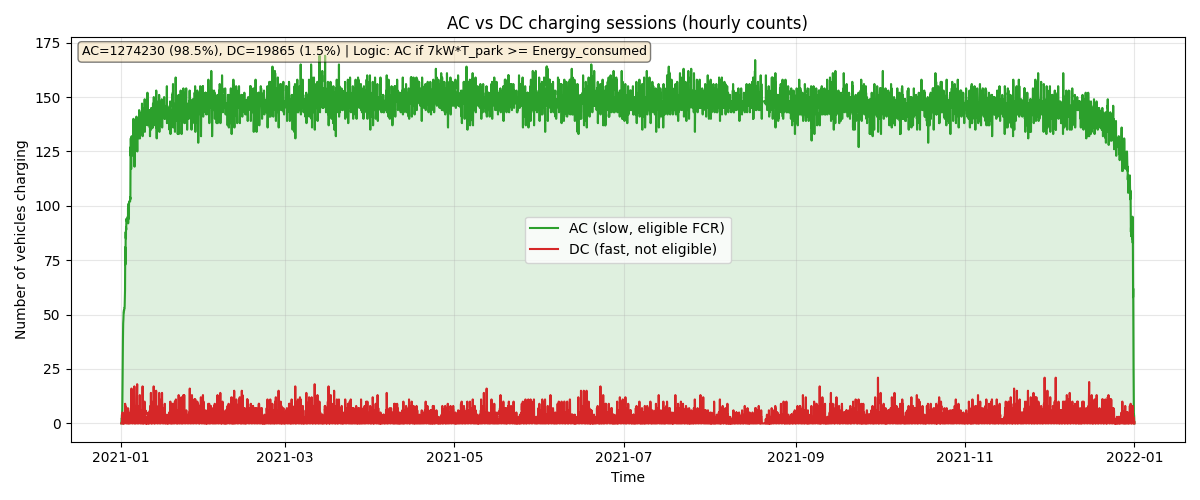
\includegraphics[width=\linewidth]{pictures/Histogramme Q8.png}
    \caption{Distribution of Charging Sessions (Q8). 98.5\% are AC-compatible, maximizing the fleet's V2G availability.}
    \label{fig:q8_dist}
\end{figure}

\subsection{Coincidence Factor Analysis (Q9)}
The aggregator's marketable power capacity $P_{bid}$ is constrained by the \textit{coincidence factor}: the minimum number of EVs simultaneously plugged in (AC) and available over a contracting block. We computed this factor for both 1-hour and 4-hour market blocks over the entire year.

Figure \ref{fig:q9_coincidence} illustrates that, excluding the start and end of the dataset, the fleet maintains a high and stable availability (fluctuating between 120 and 145 vehicles for a fleet of 150).
\begin{figure}[H]
    \centering
    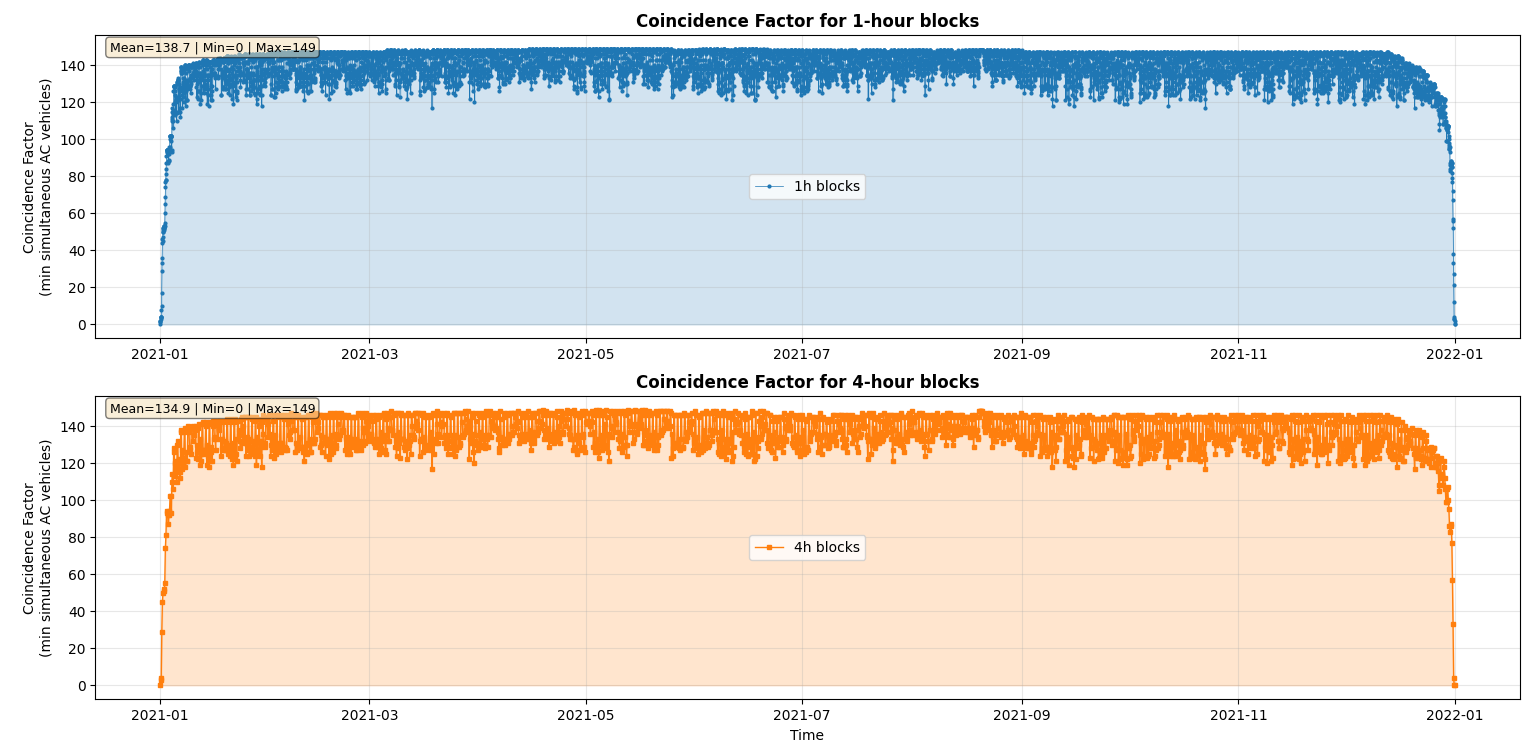
\includegraphics[width=\linewidth]{pictures/q9_coincidence.png}
    \caption{Coincidence Factor for 1-hour and 4-hour blocks over the year (Q9).}
    \label{fig:q9_coincidence}
\end{figure}

This continuous availability is a key enabler for the FCR service. It guarantees that the aggregator always possesses a sufficient "buffer" of connected vehicles. Furthermore, this high redundancy supports the \textbf{Smart dispatch strategy}: there is always a large pool of available vehicles, allowing the algorithm to select only a small subset to operate at high efficiency while letting the majority rest.

\subsection{Limitations of Inference (Q10)}
As observed in Figure \ref{fig:q9_coincidence}, the coincidence factor collapses to zero at the immediate boundaries of the year (early January and late December). This is an artifact of the simulation methodology rather than a physical reality.

\begin{itemize}
    \item \textbf{Start of Year (Ramp-up):} The inference algorithm detects a plugged-in vehicle only after a driving session ends. Consequently, vehicles that were already parked and plugged in before January 1st are "invisible" to the model until they complete their first trip of the year.
    \item \textbf{End of Year (Drop-off):} Similarly, trips ending just before the data cutoff may infer charging sessions that extend into the unknown next year. The sliding window calculation (especially the 4-hour block) encounters missing data, forcing the minimum availability to zero.
\end{itemize}

These "edge effects" artificially reduce the calculated bid capacity for the first and last weeks. In a real-world continuous operation, this limitation would not exist.

\section{Economic Assessment}

\subsection{FCR revenues (Q11)}
FCR participation is remunerated on a \textit{capacity market}: the aggregator is paid for reserving a power capacity $P_{bid}$ over each settlement block, regardless of the net energy exchanged. The bid capacity is constrained by the coincidence factor, i.e. the number of EVs simultaneously plugged in AC over the block. For a given block:
\begin{equation}
    P_{\max}(t) = 7\,N_{\text{avail}}(t) \quad [\text{kW}], \qquad
    P_{bid}(t) = \frac{P_{\max}(t)}{1.1}.
\end{equation}
Using the settlement capacity price $\pi(t)$ (in \euro/MW) from \texttt{regelleistung.net}, the revenue for the block is:
\begin{equation}
    R(t) = \pi(t)\,\frac{P_{bid}(t)}{1000}.
\end{equation}

We evaluate two market designs: (i) a \textbf{4-hour block} design (current market), and (ii) a hypothetical \textbf{1-hour block} design (future evolution). Since our price dataset is provided for 4-hour products, an equivalent hourly price is approximated as $\pi_{1h}\approx \pi_{4h}/4$.
For January 2021, the resulting monthly revenues are:
\begin{equation}
    R_{1h} = 17.76~\text{\euro/EV/month}, \qquad
    R_{4h} = 17.11~\text{\euro/EV/month}.
\end{equation}

\subsection{Virtual mileage induced by FCR (Q12)}
Although revenues are capacity-based, frequency regulation induces continuous bidirectional power exchanges. The associated absolute energy throughput is:
\begin{equation}
    E_{\text{thru}} = \int |P_{RE}(t)|\,dt.
\end{equation}
With the reduced activation signal $y_{red}(t)=5(f(t)-f_n)$ and $P_{RE}(t)=P_{bid}(t)\,y_{red}(t)$, we convert throughput into an equivalent driving distance using a driving consumption of 0.2~kWh/km:
\begin{equation}
    d_{\text{virt}} = \frac{E_{\text{thru}}}{0.2}.
\end{equation}
As frequency deviations exhibit similar statistics throughout the year, the frequency dataset and the availability dataset do not need to cover the same calendar month; the estimate relies on throughput statistics rather than exact timestamp alignment.
The resulting virtual mileage is:
\begin{equation}
    d_{\text{virt},1h}=1536.44~\text{km/EV}, \qquad
    d_{\text{virt},4h}=1474.57~\text{km/EV}.
\end{equation}

\subsection{Depreciation and net revenues (Q13)}
Virtual mileage reduces the residual value of the vehicle. Using the residual value curve $V(m)$ from \texttt{data/residual\_value.csv}, the depreciation induced by an additional mileage $d_{\text{virt}}$ for a baseline mileage $m$ is:
\begin{equation}
    \Delta V(m) = V(m) - V(m + d_{\text{virt}}).
\end{equation}
We simulate baseline mileages from 5,000~km to 75,000~km with 5,000~km steps and compute the average depreciation loss. We obtain:
\begin{equation}
    \overline{\Delta V}_{1h}=13.55~\text{\euro/EV}, \qquad
    \overline{\Delta V}_{4h}=13.00~\text{\euro/EV}.
\end{equation}
Finally, the net monthly revenue after depreciation is:
\begin{equation}
    R_{\text{net}} = R - \overline{\Delta V},
\end{equation}
leading to:
\begin{equation}
    R_{\text{net},1h}=4.21~\text{\euro/EV/month}, \qquad
    R_{\text{net},4h}=4.11~\text{\euro/EV/month}.
\end{equation}

\begin{figure}[H]
    \centering
    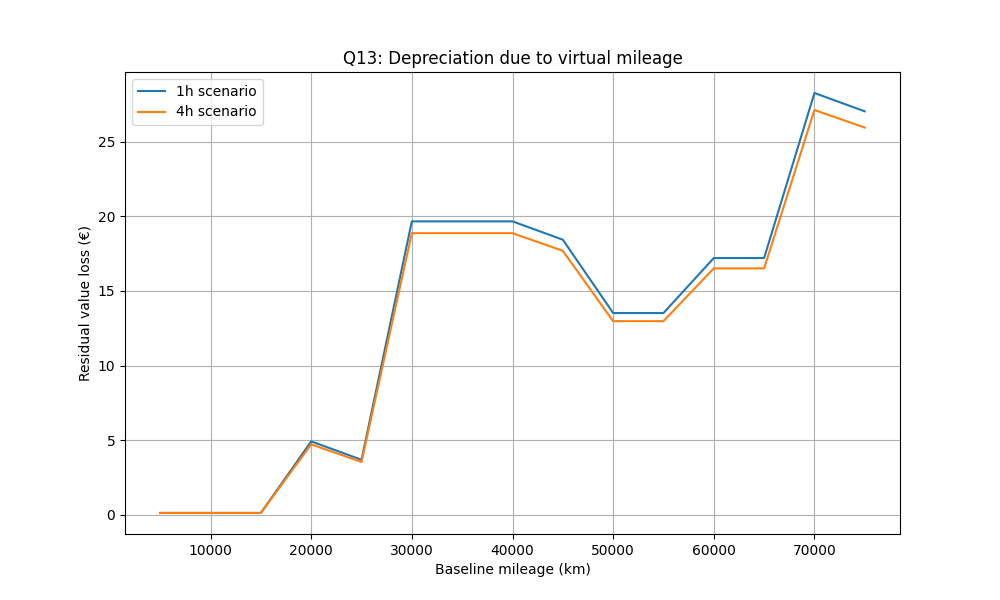
\includegraphics[width=\linewidth]{pictures/q13_residual_value_loss.png}
    \caption{Residual value loss due to virtual mileage as a function of baseline mileage (Q13).}
    \label{fig:q13_depr}
\end{figure}

Figure \ref{fig:q13_depr} shows that the additional virtual mileage induced by FCR participation leads to a non-negligible residual value loss, increasing with the baseline mileage. The 1-hour scenario results in slightly higher depreciation than the 4-hour case due to a larger effective bid capacity. Overall, battery depreciation absorbs a large share of gross revenues, reducing net profits to about $4~\euro/EV/month$.

\section{Simulation Results}

\subsection{Strategy Comparison (Q14)}
We simulated individual SOC profiles. Figure \ref{fig:comparison} highlights the fundamental difference between strategies for a single vehicle (Car 0) over the same period:
\begin{itemize}
    \item \textbf{Uniform (Top):} Smooth, continuous low-power adjustments.
    \item \textbf{Smart (Bottom):} Sharp, high-power pulses (bang-bang type control).
\end{itemize}

\begin{figure}[H]
    \centering
    \begin{subfigure}[b]{1.0\linewidth}
        
\includegraphics[width=\linewidth]{pictures/q14_soc_uniform_4h.png}
        \caption{Uniform Strategy (Car 0)}
    \end{subfigure}
    \hfill
    \begin{subfigure}[b]{1.0\linewidth}
        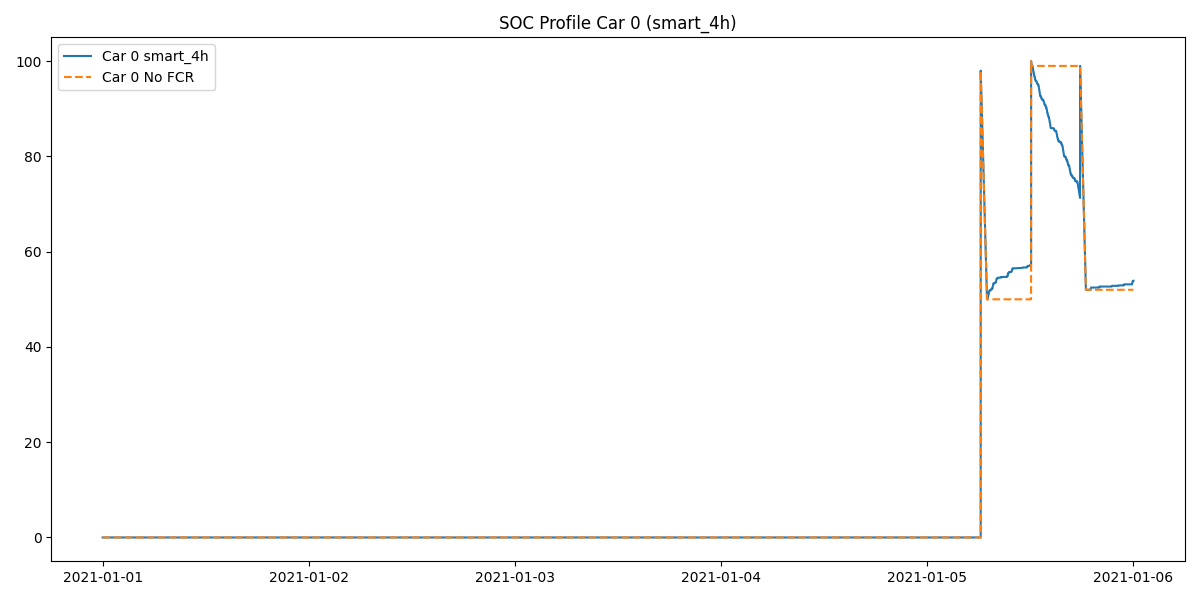
\includegraphics[width=\linewidth]{pictures/q14_soc_smart_4h.png}
        \caption{Smart Strategy (Car 0)}
    \end{subfigure}
    \caption{Comparison of SOC profiles. The Smart strategy induces higher instantaneous currents.}
    \label{fig:comparison}
\end{figure}

At the fleet level, Figure \ref{fig:agg_energy} confirms that the total energy stored follows the grid requirements identically for both strategies, validating the aggregation logic.

\begin{figure}[H]
    \centering
    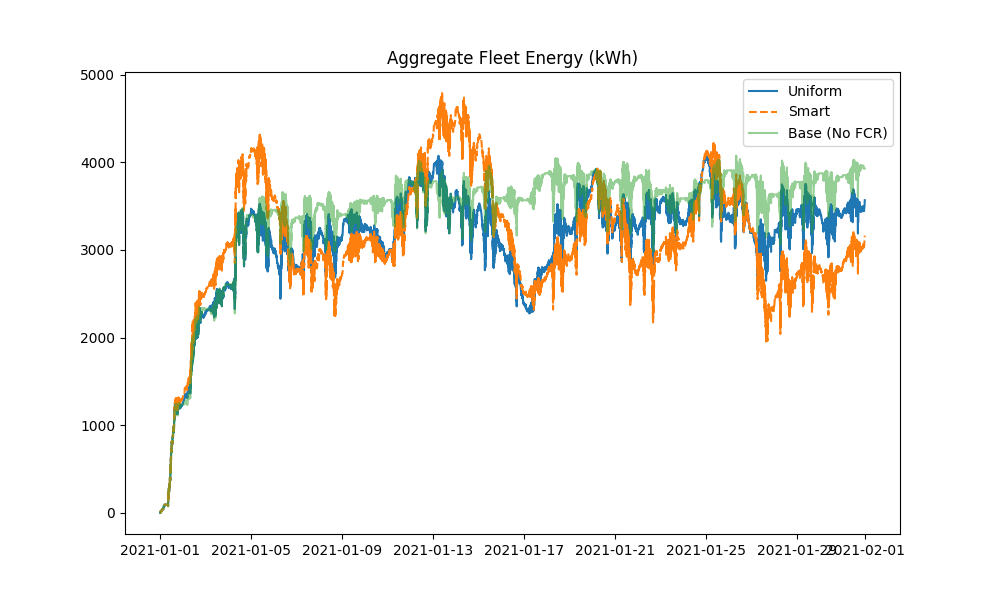
\includegraphics[width=\linewidth]{pictures/sim_aggregate_energy.png}
    \caption{Aggregate Fleet Energy evolution comparison.}
    \label{fig:agg_energy}
\end{figure}

\section{Battery Degradation Modelling}

\subsection{Battery Electrical Model (Q15)}
To evaluate battery ageing, we must first determine the internal current $I$ generated by the power demand $P$. The battery is modelled using a Thévenin equivalent circuit, consisting of an open-circuit voltage source ($OCV$) in series with an internal resistance ($R$).

\begin{figure}[H]
    \centering
    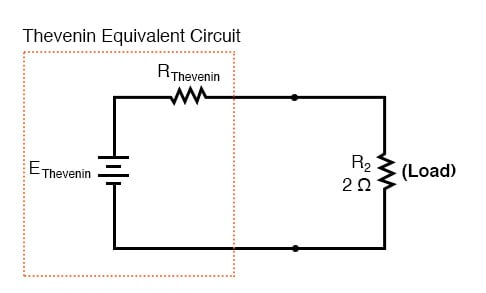
\includegraphics[width=0.8\linewidth]{pictures/Thervenin_Equivalent.jpg}
    \caption{Thevenin Equivalent Circuit model for the battery.}
    \label{fig:thevenin}
\end{figure}

\subsubsection{Derivation of the Current-Power Relationship}
Let $U_{term}$ be the terminal voltage and $P$ the power at the battery terminals. By convention, we assume $P>0$ corresponds to discharging. The circuit is governed by Kirchhoff's voltage law:
\begin{equation}
    U_{term} = OCV - R \cdot I
\end{equation}
The power exchanged at the terminals is defined as:
\begin{equation}
    P = U_{term} \cdot I
\end{equation}
By substituting (5) into (6), we obtain:
\begin{equation}
    P = (OCV - R \cdot I) \cdot I = OCV \cdot I - R \cdot I^2
\end{equation}
Rearranging this terms leads to a quadratic equation for the current $I$:
\begin{equation}
    R \cdot I^2 - OCV \cdot I + P = 0
\end{equation}
The solutions are given by the quadratic formula:
\begin{equation}
    I = \frac{OCV \pm \sqrt{OCV^2 - 4 \cdot R \cdot P}}{2R}
\end{equation}
To determine the physically correct root, we consider the idle state. When $P=0$, the current must be zero ($I=0$).
\begin{itemize}
    \item Case $(+)$: $I = \frac{2 \cdot OCV}{2R} = \frac{OCV}{R}$ (Short-circuit current, physically incorrect).
    \item Case $(-)$: $I = \frac{0}{2R} = 0$ (Correct).
\end{itemize}
Thus, the current $I$ as a function of power is:
\begin{equation}
    I(P) = \frac{OCV - \sqrt{OCV^2 - 4 \cdot R \cdot P}}{2R}
\end{equation}

\vspace{0.5em}
\section{Conclusion}
This study investigated the participation of electric vehicle (EV) fleets in Primary Frequency Containment Reserves (FCR), combining grid frequency modelling, fleet dispatch strategies, battery ageing analysis, and economic assessment.

The results demonstrate that a Smart dispatch strategy significantly improves energy conversion efficiency (≈95\% compared to ≈86\% under uniform allocation) and drastically reduces on-board charger operating time. However, this gain is achieved by concentrating power on a subset of vehicles, leading to higher instantaneous battery currents and increased degradation (+7.5\% versus +2.8\%).

Despite this accelerated ageing effect, the economic evaluation confirms that FCR participation remains financially viable, as capacity revenues compensate for the depreciation induced by virtual mileage.

These findings indicate that EV fleets can provide frequency containment services without compromising asset value, provided that dispatch strategies account for battery stress and operational constraints.

Future work should integrate more advanced ageing models (including cycle counting and calendar ageing effects) and explore optimization-based degradation-aware dispatch algorithms to further enhance long-term economic performance.

In the context of increasing renewable penetration and declining system inertia, aggregated EV fleets emerge as a scalable and distributed flexibility resource capable of supporting grid stability.

\end{document}